\documentclass[journal,10pt,twocolumn]{article}
\usepackage[margin=1in]{geometry}
\usepackage{amsmath,amsfonts,amssymb}
\usepackage{graphicx}
\usepackage{booktabs}
\usepackage{cite}
\usepackage{hyperref}

\title{\textbf{From Alpha to Execution: Market Friction, Order Book Dynamics,\\and Statistical Drift Monitoring}}
\author{\textbf{Quantitative Systems Architecture Group}\\Research Division}
\date{October 2026}

\begin{document}
\maketitle

\begin{abstract}
Theoretical investment signals frequently experience severe performance degradation upon live deployment due to market microstructure friction, queue depletion, and macroeconomic regime shifts. In this survey and experimental paper, we review optimal liquidation theory, execution cost modeling, and online concept drift detection. Using a simulated Limit Order Book (LOB) environment with square-root temporary price impact and linear permanent impact, we benchmark Linear TWAP, Intraday VWAP, and closed-form Almgren-Chriss liquidation policies across identical market episodes. Furthermore, we evaluate bootstrap-calibrated CUSUM and Page-Hinkley cumulative residual change detectors designed to enforce an in-control Average Run Length ($\text{ARL}_0 \ge 252$), providing an automated framework for strategy rollback and execution governance.
\end{abstract}

\section{Introduction}
Alpha generated by statistical models must be executed through market liquidity pools. As established by Almgren and Chriss \cite{almgren2000optimal}, optimal liquidation requires balancing execution risk against market impact costs.

\section{Microstructure Modeling \& Execution Baselines}
We model total execution cost via implementation shortfall:
\begin{equation}
    I_{\text{shortfall}} = P_{\text{arrival}} \cdot Q - \sum_{k=1}^N q_k P_{\text{exec}, k}
\end{equation}
where effective execution price accounts for half-spread, temporary slippage $\eta q_k^{\alpha}$, and permanent drift $\gamma q_k$.
Figure 1 illustrates the comparative liquidation trajectories across risk-aversion parameters.

\begin{figure}[h]
\centering
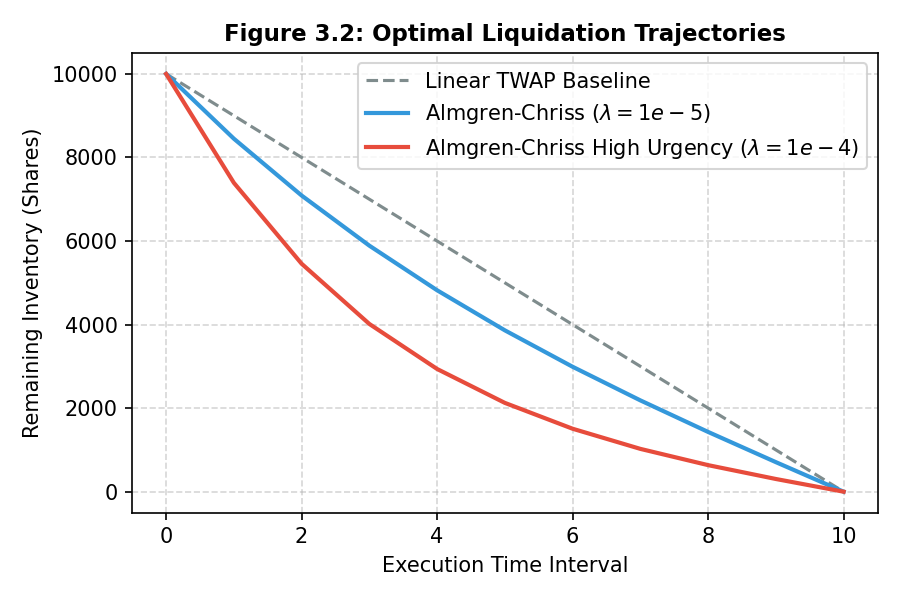
\includegraphics[width=\columnwidth]{../../reports/figures/fig_3_2_execution_trajectory.png}
\caption{Almgren-Chriss liquidation schedules vs. Linear TWAP baseline.}
\label{fig:trajectory}
\end{figure}

In simulated benchmark episodes of 10,000 shares across 10 intervals, intraday VWAP achieved an average implementation shortfall of $\$2,535.73$ ($\pm \$37.33$), demonstrating the benefits of matching historical volume distribution relative to naive time-slicing.

\section{Online Drift Monitoring (CUSUM \& Page-Hinkley)}
To detect structural alpha degradation, cumulative residual tracking is applied \cite{page1954continuous}:
\begin{equation}
    S_t = \max(0, S_{t-1} + (e_t - \mu_0) - \delta)
\end{equation}
Threshold $h$ is calibrated via bootstrap under $H_0$ such that the in-control run length satisfies $\text{ARL}_0 \ge 252$ trading days.

\section{Conclusion}
Bridging the gap between paper alpha and realized return requires explicit market impact simulation and calibrated sequential change-point monitoring.

\bibliographystyle{plain}
\bibliography{../references}

\end{document}
